\chapter{Deep Learning Modelle im Web}\label{ch8}
Das Modell muss in einer Art und Weise für den Nutzer (Client) zugänglich gemacht werden. Das Modell welches in dieser Arbeit entwickelt wurde, kann nur Zahlen verstehen. Es muss also in erster Linie ein Encoder die Strings in Zahlen umwandeln. Je nach Plattform findet erst dann die Berechnung der Vorhersage statt. Im ersten teil dieses Kapitels wird eine klassische \enquote{serverseitige} Implementierung vorgenommen. Diese dient zu Demonstrationszweck und benötigt keine UI. Es wird lediglich ein HTTP-Endpunkt programmiert, welches eine JSON-Anfrage in ein Modell weitergibt und dann die entsprechende Antwort wieder als Antwort zurück gibt. Im Anschluss darauf wird die in dieser Arbeit vorgeschlagene Methode des clientseitigen Deep Learnings vorgestellt. Beide Methoden haben Ihre Vor- und Nachteile, diese werden anschließend analysiert.

\section{Serverseitiges Deep Learning}
Um das Deep Learning auf der Seite des Servers auszuführen wird ein Server geschrieben. Auf diesem Server läuft das Modell und wartet auf die Anfragen, die auf den Endpunkt \texttt{/predict} zukommen. Ein solcher Server kann mittels der Bibliothek Flask in Python programmiert werden. Der Server hat nur eine Route, diese Route wartet auf einen JSON-POST-Request. Nachdem der Server diese JSON-Information aufgenommen hat, kann er den Text in das Modell weitergeben. Da das Modell nur Zahlen versteht, ist das Encoden der Texte erforderlich. Die Methoden die hier verwendet werden sind sehr ähnlich zu den Methoden, die beim Trainieren verwendet wurden. Aus diesem Grund wird nicht näher auf diese eingegangen  (vgl. Listing \ref{Server} mit Abschnitt \ref{vocSec}).

\begin{lstlisting}[language=Python,caption=Beispiel eines Servers für die Vorhersage von Clickbaits, label={Server}]
from flask import Flask, request
from keras.preprocessing.text import tokenizer_from_json
from keras.preprocessing.sequence import pad_sequences
from keras.models import load_model
from flask import request
import numpy as np
import json


app = Flask(__name__)
max_len = 40
labels = np.array(["Clickbait", "News"])
model = load_model("model/model.h5")
with open("model/tokenizer.json") as f:
    tokenizer = tokenizer_from_json(json.load(f))


def encode(text):
    return pad_sequences(tokenizer.texts_to_sequences(text), maxlen=40)


@app.route("/predict", methods=["POST"])
def postJsonHandler():
    if request.method == "POST":
        return json.dumps({"prediction": labels[np.argmax(model.predict(encode([request.get_json()["text"]])))]})

        
if __name__ == "__main__":
    app.run()
\end{lstlisting}




\section{Clientseitges Deep Learning}
Dieser Abschnitt beschäftigt sich mit dem clientseitigen Deep Learning. Um TensorFlow.js praktisch anzuwenden wurde in React\footnote{React ist ein Frontend Framework für JavaScript. Es wurde von Facebook entwickelt und ist Open Source.} ein Frontend entwickelt, welches vom Modell Gebrauch macht. Für eine Inferenz ist ein Server nicht mehr nötig. Alleine der Zugriff auf die \textt{model.json} Datei und die jeweiligen Gewichte reichen für diese Variante aus. Die Dateien werden auf einem Server von AWS\footnote{Amazon Web Services (AWS) ist eine Cloud-Service-Plattform, die Rechenleistung, Datenbankspeicher, Bereitstellung von Inhalten und andere Funktionen bietet.} gehostet und können in den Browser geladen werden. Das Frontend wird außerdem die gesamte TensorFlow.js Bibliothek in den Browser laden. Da die gesamte Inferenz im Browser stattfindet, muss auf die Größe des Modells geachtet werden. Das in dieser Arbeit entwickelte Modell ist mit seiner gesamten Größe von ca. 3 MB relativ klein. Die Ordnerstruktur aus Listing \ref{OrdnerStr} ist ein Ausschnitt der Frontend Ordnerstruktur und soll in den nächsten Abschnitten beschrieben werden. Somit kann ein Verständnis über die Zusammenhänge zwischen Deep Learning und Webanwendung erläutert werden.

\begin{lstlisting}[language=bash,caption=Wichtigste Elemente der Benutzeroberfläche, label={OrdnerStr}]
|____src
| |____constants
| | |____constants.js
| |____hooks
| | |____index.js
| | |____useLoadVocab.js
| | |____useLoadModel.js
| |____helpers
| | |____splitText.js
| | |____index.js
| | |____tokenize.js
| |____index.js
| |____App.js
\end{lstlisting}

\section{Tokenisierung und Padding}
Unter dem Verzeichnis \enquote{helpers} befinden sich die Skripte zur Erstellung der Tokens. Der von dem User eingegebene Text muss in seine Tokens zerlegt werden und außerdem muss die Interpunktion gefiltert werden (außer Ausrufezeichen und Fragezeichen). Ein Wort darf außerdem nicht weniger als ein Zeichen enthalten und außerdem müssen die Wörter in Kleinbuchstaben umgewandelt werden, da die \textt{vocab.json} nur solche enthält. Im Listing~\ref{splitText} wird die Funktion dargestellt, welches den Satz, dass der Nutzer eingibt in Token umwandelt. Hier wird ein vorprogrammierter Tokeniser\footnote{https://www.npmjs.com/package/wink-tokenizer} verwendet, welches die Tokens auch taggen kann (Zahl, Wort usw.). Die Tokens werden entsprechend gefiltert und und als Array zurückgegeben. Das Ergebnis dieser Prozedur muss der Prozedur aus der Python Umgebung gleichen und möglichst ähnliche Ergebnisse zurück geben, sonst wird das Modell in der Praxis etwas anderes zugeteilt bekommen als vorgesehen. 

\begin{lstlisting}[language=JavaScript, caption=Die splitText Funktion, label={splitText}]
const tokenizer = require('wink-tokenizer');
const myTokenizer = tokenizer();

const splitText = (sentence) => {
  const tokens = myTokenizer.tokenize(sentence);
  const splitted = [];
  tokens.forEach((token) => {
    if (token.tag === 'number') {
      splitted.push(token.value);
    } else if (token.tag === 'word') {
      if (token.value.length >= 1) {
        splitted.push(token.value.toLowerCase());
      }
    } else if (token.tag === 'punctuation') {
      if (token.value === '?' || token.value === '!') {
        splitted.push(token.value);
      }
    }
  });

  return { splitted: splitted, splittedLen: splitted.length };
};

export default splitText;
\end{lstlisting}

Im nächsten Schritt müssen die Tokens in Zahlen umgewandelt werden. In der Python Umgebung wurde dies mit der Methode \texttt{pad\_sequences} aus der Keras-Bibliothek ausgeführt. In JavaScript gibt es keinen Ersatz für diese Methode, sodass es selbst programmiert wird. Die \texttt{tokenize}-Funktion nimmt den Text den der Client eingibt und führt diese in die \texttt{splitText}-Funktion ein. Für alle Tokens wird ein Abgleich mit der \texttt{vocab.json} erstellt und wenn ein Treffer gefunden wurde, der Index in eine Array eingeführt. Die maximale Länge wird später aus der Datei \texttt{constants.js} entnommen und beträgt in diesem Beispiel 40. Damit entsteht ein Array der Länge 40, mit \textit{n} Treffern und \textit{40-n} Nullen. Der Parameter \texttt{vocabLoading} ist ein Boolean, welches aussagt, ob die \texttt{vocab.json} aktuell geladen wird oder nicht. Diese Datei (genauso wie die \texttt{model.json} und die Gewichte) werden in asynchron geladen. Dieses Laden kann in JavaScript den gesamten Prozess blockieren. Um dieses zu vermeiden werden sogenannte \enquote{Promises} verwendet. Das Promise-Objekt repräsentiert in JavaScript den eventuellen Abschluss (oder Fehler) einer asynchronen Operation und den daraus resultierenden Wert.


\begin{lstlisting}[language=JavaScript, caption=Die tokenize Funktion, label={tokenizejs}]
import splitText from './splitText';

const tokenize = (text, vocabLoading, vocab, maxLen) => {
  const { splitted } = splitText(text);
  const tokens = [];

  if (!vocabLoading) {
    splitted.forEach((element) => {
      if (vocab[element] !== undefined) {
        tokens.push(vocab[element]);
      }
    });

    while (tokens.length < maxLen) {
      tokens.push(0);
    }
  }
  return tokens.slice(0, maxLen);
};

export default tokenize;
\end{lstlisting}

\section{Laden des Modells und Vokabulars}
Die Dateien für das Modell und die jeweiligen Gewichte wie ebenfalls die Datei für das Vokabular wurden in AWS gehostet. Um diese Dateien in den Browser zu laden wurden \enquote{Hooks} (ähnlich wie Funktionen) in React geschrieben. Der Grund dafür ist, dass dadurch eine Abstraktion dieser Prozesse stattfindet und diese Prozesse von dem eigentlichen Prozess der Erstellung einer Benutzeroberfläche getrennt werden. Damit lassen sie sich im Hauptprozess einfach aufrufen, und der Konsument dieser Funktion muss nicht mehr wissen, wie diese Daten geladen werden können. Damit sind diese Prozesse wiederverwendbar und leichter zu kontrollieren.
Im wesentlichen wird aber in der Funktion \ref{useLoadModel} das Modell geladen (ähnlich wird auch das Vokabular geladen). Das Modell wird in eine Variable \texttt{model} gespeichert. Wenn das Modell noch lädt, wird dieses ebenfalls in eine Variable \texttt{modelLoading} gespeichert. Diese beiden Variablen werden der gesamten UI mitgeteilt. Somit können alle Komponenten diesen Status wissen und darauf reagieren. Durch das Einbinden von TensorFlow.js in die UI, hat der Client vollen Zugriff  TensorFlow. Mit der Methode \texttt{loadLayersModel} kann ein Modell geladen werden, welches aus mehreren Ebenen besteht, einschließlich seiner Gewichte. Die Methode \texttt{ready} gibt ein Promise zurück, welches aufgelöst wird, wenn das aktuell ausgewählte Backend initialisiert wurde. Es findet also eine \enquote{asynchrone Initialisierung} statt. Die Ausgabe der \texttt{useLoadModel} Hook ist das Modell einschließlich aller anderen Variablen im Zusammenhang mit dem Laden des Modells.


\begin{lstlisting}[language=JavaScript, caption=Das useLoadModel Hook, label={useLoadModel}]
import { useState, useEffect } from 'react';
import * as tf from '@tensorflow/tfjs';

const useLoadModel = (url) => {
  const [model, setModel] = useState();
  const [modelLoading, setModelLoading] = useState(true);
  const [modelError, setModelError] = useState('');
  
  const loadModel = async (url) => {
    try {
      const model = await tf.loadLayersModel(url);
      setModel(model);
      setModelLoading(false);
    } catch (error) {
      setModelError(error);
      setModelLoading(true);
    }
  };

  useEffect(() => {
    tf.ready().then(() => {
      loadModel(url);
    });
  }, [url]);

  return {
    model,
    setModel,
    modelLoading,
    setModelLoading,
    modelError,
    setModelError,
  };
};

export default useLoadModel;
\end{lstlisting}

\section{Die Vorhersage des Modells}
Die \texttt{predict}-Funktion wird in der Datei \texttt{App.js} aufgerufen und ist somit die Funktion, welches aufgerufen wird, wenn ein Ereignis stattfindet (der Nutzer auf den Button klickt). Die API von TensorFlow.js bietet eine Methode Namens \texttt{tidy} welches die bereitgestellte Funktion ausführt und nach der Ausführung alle von der Funktion zugewiesenen Zwischentensoren mit Ausnahme der Funktion vom Speicher entleert. Mit dieser Methode können Speicherleaks vermieden werden. Ein Array mit den Tokens wird in ein 2-dimensionales Tensor umgewandelt und geht durch das Modell. Mit \texttt{dispose} wird der Tensor dann am Ende aus dem Speicher entsorgt. In Abbildung \ref{Frontend} befindet sich die UI.

\begin{lstlisting}[language=JavaScript, caption=Auszug aus der predict Funktion, label={prediJS}]
const predict = async () => {
    const predictedClass = await tf.tidy(() => {
      const tokenisation = tokenize(inputText, vocabLoading, vocab, maxLen);
      if (tokenisation.length > 0) {
        const input = tf.tensor2d(tokenisation, [1, maxLen]);
        if (!modelLoading) {
          const predictions = model.predict(input);
          return predictions.as1D().argMax();
        }
      }
    });
  };
\end{lstlisting}


\begin{figure}[H]
    \centering
    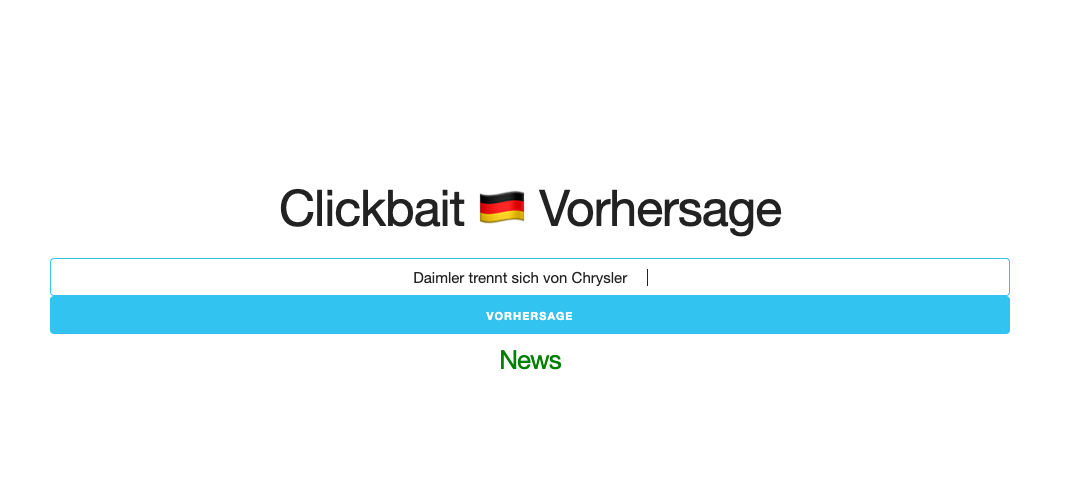
\includegraphics[width=14cm]{kapitel5/frontend.png}
    \caption[Das Frontend]{Die Benutzeroberfläche, welches im Hintergrund mit dem Deep Learning Modell kommuniziert.}
    \label{Frontend}
\end{figure}

\section{Vergleich beider Ansätze}


In diesem Abschnitt sollen die Ansätze \enquote{serverseitiges Deep Learning} und \enquote{clientseitiges Deep Learning} verglichen werden. Beide Ansätze haben Ihre Vor- und Nachteile. Die Vorteile für das clientseitige Deep Learning sind, dass es geringe Serverkosten hat, die Inferenzlatenz geringer ist und eine Datenprivatsphäre gewährleistet ist. 

\textit{Serverkosten} spielen beim Entwerfen und Skalieren von Webdiensten eine wichtige Rolle. Häufig müssen GPU Server bereitgestellt  \cite[19]{cai2020deep}. Beim clientseitigen Deep Learning muss ein kleines Modell (in diesem Beispiel ca. 3 MB groß) bereitgestellt werden und daraus kann die Inferenz stattfinden.

Ein weiterer Punkt ist die \textit{Inferenzlatenz}. Für bestimmte Arten von Anwendungen ist die Latenz Anforderung so hoch, dass die Deep-Learning-Modelle auf der Clientseite ausgeführt werden sollten. Alle Anwendungen, die Audio-, Bild- und Videodaten in Echtzeit enthalten, fallen in diese Kategorie. Wenn Daten erst auf ein Server geladen werden müssen um dann eine Antwort zu erhalten, steigt somit auch die Latenzzeit. Die clientseitige Inferenz behebt diese potenziellen Latenz- und Konnektivitätsprobleme, indem die Daten und die Berechnung auf dem Gerät gespeichert werden \cite[20]{cai2020deep}. Bei NLP Anwendungen ist dieses kein großer Argument, da Textdaten meistens kleiner sind, ist die Inferenzlatenz auch geringer.

\textit{Datenschutz} ist ein weiterer Vorteil des clientseitigen Deep Learnings. Das Thema Datenschutz wird heute immer wichtiger. Für bestimmte Arten von Anwendungen ist Datenschutz eine absolute Voraussetzung. Anwendungen in Bezug auf Gesundheits- und medizinische Daten sind ein prominentes Beispiel. In vielen Ländern erlauben die Datenschutzbestimmungen für Gesundheitsinformationen nicht, dass z.B. Bilder auf einen zentralen Server übertragen werden. Ein weiteres Szenario könnten juristische Dokumente sein, die nicht auf ein drittes Server geladen werden sollten \cite[20]{cai2020deep}. 

Für \textit{größere Modelle} eignet sich das clientseitige Deep Learning nicht, da es für den Nutzer nicht praktisch ist, ein Modell mit mehreren GB Größe, in den Browser zu laden. Ein weiterer Vorteil für das serverseitige Deep Learning ist, dass \textit{Python} als Programmiersprache wesentlich reifer ist, als JavaScript, wenn es um Deep Learning geht. 